\documentclass[11pt]{article}

\usepackage{extsizes}
\usepackage{graphicx} % Required for inserting images
\graphicspath{ {./} }
\usepackage{svg}
\usepackage{doi}
\usepackage{wrapfig}

\usepackage[style=ieee]{biblatex}
\addbibresource{bibliography.bib}


%\usepackage{navigator}
%\embeddedfile{knapsack}{knapsack.py}

% All needed for attachfile (oroginal)
% Gah! lualatex renamed primatives so this fixes it:
%\let\pdfxform\saveboxresource
%\let\pdfximage\saveimageresource
%\let\pdfrefxform\useboxresource
%\let\pdfrefximage\useimageresource
%\let\pdflastxform\lastsavedboxresourceindex
%\let\pdflastximage\lastsavedimageresourceindex
%\let\pdflastximagepages\lastsavedimageresourcepages
% https://www.tug.org/pipermail/luatex/2017-July/006592.html
% http://mirrors.ibiblio.org/CTAN/systems/doc/luatex/luatex.pdf, page44

% Also enable pdfannot 
%\protected\def\pdfannot {\pdfextension annot}

%\usepackage{attachfile2}





\usepackage[a4paper, margin=1in]{geometry}
\usepackage{hyperref}

% \usepackage{changepage}
\usepackage{parskip}
\usepackage{fontspec}
%\usepackage{amsfonts}

\usepackage{embedfile}
\usepackage{hypgotoe}

%\embedfile{data-visualisation.py}
%\embedfile{mariner-david-davies/data0.json}
%\embedfile{ship-adroit/data0.json}
%\embedfile{ship-catherine-morgan/data0.json}

\usepackage{listingsutf8}
\usepackage{xcolor}

\definecolor{codegreen}{rgb}{0,0.6,0}
\definecolor{codegray}{rgb}{0.5,0.5,0.5}
\definecolor{codepurple}{rgb}{0.58,0,0.82}
\definecolor{backcolour}{rgb}{0.95,0.95,0.95}
\definecolor{backconsolecolour}{rgb}{0.2,0.2,0.2}
\definecolor{codered}{rgb}{0.95,0.31,0.31}
\definecolor{codeblue}{rgb}{0.16,0.5,0.72}

\lstdefinestyle{code}{
    backgroundcolor=\color{backcolour},   
    commentstyle=\color{codegreen},
    keywordstyle=\color{magenta},
    numberstyle=\tiny\color{codegray},
    stringstyle=\color{codepurple},
    basicstyle=\ttfamily\footnotesize,
    breakatwhitespace=false,         
    breaklines=true,                 
    captionpos=b,                    
    keepspaces=true,                 
    numbers=left,                    
    numbersep=5pt,                  
    showspaces=false,                
    showstringspaces=false,
    showtabs=false,                  
    tabsize=2
}

\lstdefinestyle{console}{
    backgroundcolor=\color{backconsolecolour},   
    commentstyle=\color{codegreen},
    keywordstyle=\color{magenta},
    numberstyle=\tiny\color{codegray},
    stringstyle=\color{codepurple},
    basicstyle=\ttfamily\footnotesize\color{white},
    breakatwhitespace=false,         
    breaklines=true,                 
    captionpos=b,                    
    keepspaces=true,                 
    numbers=left,                    
    numbersep=5pt,                  
    showspaces=false,                
    showstringspaces=false,
    showtabs=false,                  
    tabsize=2
}

\lstdefinelanguage{json}{
    basicstyle=\normalfont\ttfamily,
    commentstyle=\color{codered}, % style of comment
    stringstyle=\color{codeblue}, % style of strings
    showstringspaces=false,
    breaklines=true,
    backgroundcolor=\color{backcolour}, %only if you like
    string=[s]{"}{"},
    comment=[l]{:\ "},
    morecomment=[l]{:"},
    literate=
        *{0}{{{\color{numb}0}}}{1}
         {1}{{{\color{numb}1}}}{1}
         {2}{{{\color{numb}2}}}{1}
         {3}{{{\color{numb}3}}}{1}
         {4}{{{\color{numb}4}}}{1}
         {5}{{{\color{numb}5}}}{1}
         {6}{{{\color{numb}6}}}{1}
         {7}{{{\color{numb}7}}}{1}
         {8}{{{\color{numb}8}}}{1}
         {9}{{{\color{numb}9}}}{1}
         {\{}{{{\color{codepurple}\{}}}{1}
         {\}}{{{\color{codepurple}\}}}}{1}
         {[}{{{\color{codegreen}[}}}{1}
         {]}{{{\color{codegreen}]}}}{1}
}

% \usepackage{floatrow}
% \usepackage[no-math]{fontspec}
\usepackage{amsmath}
\usepackage{lipsum}

\usepackage{xurl}

\title{Setting up the BRAIN project on a fresh NVIDIA Jetson AGX/Nano}
\author{Alex Baldwin}
\date{August 2025}

\begin{document}

\maketitle

\begin{abstract}

This document covers installing the BRAIN vision compute stack on an NVIDIA embedded compute device. The proceedures outlined below have been tested to work on an NVIDIA Jetson AGX Orin and an NVIDIA Jetson Orin Nano.

\end{abstract}

\tableofcontents

\newpage

\section{Prerequisites}

\subsection{Essential hardware}

When travelling with the Jetson, it's critical to be prepared with the following items for debugging:
\begin{itemize}
\item A laptop with a Debian based OS (This guide has been tested with Ubuntu 24.04 and Debian 13)
\item USB A/C to USB Micro B cable (for serial debugging)
\item USB A/C to USB C cable (USB 3.1 capable minimum) (for firmware flashing)
\item \textgreater{}128GB Micro SD card
\item SD card reader, if your laptop cannot read them directly
\item USB C Power Delivery capable power supply
\item USB Keyboard
\item Ethernet Cable
\end{itemize}

\subsection{Flashing the base OS image}

The official NVIDIA images come with a full desktop environment and a lot of other bloat. Therefore, BRAIN is currently built for a host based on the \href{https://cdimage.ubuntu.com/releases/jammy/release/nvidia-tegra/ubuntu-22.04-preinstalled-server-arm64+tegra-jetson.img.xz}{ARM64 Tegra Ubuntu Server 22.04 release}. To begin, download the image and extract it to your computer. Then use \texttt{dd} to write the image to your Micro SD card:

\lstset{style=console}
\begin{lstlisting}
alewin@NOCS000000:~$ lsblk
NAME                     MAJ:MIN RM   SIZE RO TYPE  MOUNTPOINTS
sda                        8:0    1 238.8G  0 disk
└─sda1                     8:1    1 238.7G  0 part
nvme0n1                  259:0    0 476.9G  0 disk
├─nvme0n1p1              259:1    0   512M  0 part  /boot/efi
├─nvme0n1p2              259:2    0   488M  0 part  /boot
└─nvme0n1p3              259:3    0   476G  0 part
 └─nvme0n1p3_crypt      253:0    0 475.9G  0 crypt
   ├─nocs000000--vg-root   253:1    0   475G  0 lvm   /
   └─nocs000000--vg-swap_1 253:2    0   980M  0 lvm   [SWAP]
alewin@NOCS000000:~$ sudo dd if=ubuntu-22.04-preinstalled-server-arm64+tegra-jetson.img of=/dev/sda bs=16M
[sudo] password for alewin:
323+1 records in
323+1 records out
5422220800 bytes (5.4 GB, 5.0 GiB) copied, 169.935 s, 31.9 MB/s
\end{lstlisting}

The current BRAIN stack is designed to run within docker, with host NVIDIA CUDA drivers of 12.6 or later. We target a minimum firmware version of 36.4, which is sometimes installed by default. You should check the firmware version on the UEFI BIOS screen upon first boot of your Jetson. If your firmware version is older than 36.4, you will need to follow the reflashing step detailed in \autoref{sec:debug-reflash_firmware} before continuing.

The official NVIDIA images boot the kernel driectly using ExtLinux, but the Ubuntu Server release uses GRUB. To change this setting, you must hit \textit{ESC} at startup to enter the UEFI BIOS settings, and navigate to the submenu \textit{Device Manager} \Rightarrow \textit{NVIDIA Configuration} \Rightarrow \textit{L4T Configuration} \Rightarrow \textit{L4T Boot Mode}.

\subsection*{Side note specific to the Orin AGX}

The AGX has an internal 32GB eMMC chip which is usually flashed with an old NVIDIA Ubuntu Desktop image. This can be useful to keep around, or you can re-flash it to the Ubuntu Server image as well. The AGX will want to boot from the eMMC by default, so you must hit \textit{ESC} to enter the UEFI BIOS settings, and change the default boot device to UEFI SD card. It is in the submenu \textit{Boot Maintenance Manager} \Rightarrow \textit{Boot Options} \Rightarrow \textit{Change Boot Order}.

It's not possible to install the entire BRAIN stack to the on-board storage due to space constraints, so it's reccomended to install everything to the SD card. It is possible to install the base OS on eMMC, and leave only the docker images on the SD card, but this is a more complicated install method, and is usually not worth it unless you're unable to source a \textgreater{}128GB Micro SD card.

\subsection{Setting up the base OS image}

By default, the Ubuntu Server image will attempt to mount a cloud-init config file. After about 1m30s it will abort, and create a default user with the username \texttt{ubuntu} and password \texttt{ubuntu}, and enable this account for SSH login. You will be required to change the password immediately. The fact that this image ships with cloud-init is notable, as it is actually possible to set up the BRAIN stack automatically on Jetson without a monitor at all. However, it's much easier to set up the device manually, and a monitor is a must-have for debugging when all else fails.

The Jetson will automatically connect to any LAN with DHCP on its primary Ethernet interface. You may want to use the arp-scan tool to find it on your LAN:

\lstset{style=console}
\begin{lstlisting}
alewin@NOCS000000:~$ sudo arp-scan 10.42.0.0/24
[sudo] password for alewin:
Interface: enp0s31f6, type: EN10MB, MAC: 28:00:af:74:97:0c, IPv4: 10.42.0.1
Starting arp-scan 1.10.0 with 256 hosts (https://github.com/royhills/arp-scan)
10.42.0.49      3c:6d:66:XX:XX:XX       (Unknown)

1 packets received by filter, 0 packets dropped by kernel
Ending arp-scan 1.10.0: 256 hosts scanned in 1.989 seconds (128.71 hosts/sec). 1 responded

alewin@NOCS000000:~$ ssh ubuntu@10.42.0.49
The authenticity of host '10.42.0.49 (10.42.0.49)' can't be established.
Are you sure you want to continue connecting (yes/no/[fingerprint])? yes
Warning: Permanently added '10.42.0.49' (ED25519) to the list of known hosts.
ubuntu@10.42.0.49's password:
Welcome to Ubuntu 22.04 LTS (GNU/Linux 5.15.0-1020-nvidia-tegra-igx aarch64)
[...]
Last login: Tue Nov 21 22:54:35 2023
ubuntu@brain0:~$

\end{lstlisting}

\textbf{NOTE:} If you plan to use the SD card on Jetsons other than the one it first booted in, see \autoref{sec:debug-network_config} for additional setup needed to ensure DHCP works as expected.

Start by creating a new user for deployment, adding them to \texttt{sudo} group:

\lstset{style=console}
\begin{lstlisting}
ubuntu@ubuntu:~$ sudo adduser deploy
[sudo] password for ubuntu:
New password:
Retype new password:
passwd: password updated successfully
Changing the user information for deploy
Enter the new value, or press ENTER for the default
        Full Name []: Deployer McDeployface
        Room Number []:
        Work Phone []:
        Home Phone []:
        Other []:
Is the information correct? [Y/n] Y
ubuntu@ubuntu:~$ sudo usermod -aG sudo deploy
\end{lstlisting}

\textbf{NOTE:} We use the default password \texttt{brain!} for non-networked deployments for simplicity. You MUST change this to a secure random value from \texttt{pwgen 16} or similar before deploying to a networked environment.

You should then set the hostname for the device. In order for this to fully take affect, you should reboot the device.

\begin{lstlisting}
ubuntu@ubuntu:~$ sudo hostnamectl hostname brain0
ubuntu@ubuntu:~$ sudo reboot
\end{lstlisting}

After the reboot, login with the deploy account. Now's a good time to remove \texttt{unattended-upgrades} for production systems to avoid automatic updates mid-deployment, and \texttt{cloud-init} as it's not neccesary, and can cause problems in the boot process.

\lstset{style=console}
\begin{lstlisting}
deploy@brain0:~$ sudo apt update
Hit:1 http://ports.ubuntu.com/ubuntu-ports jammy InRelease
Get:2 http://ports.ubuntu.com/ubuntu-ports jammy-updates InRelease [128 kB]
[...]
Fetched 18.4 MB in 4s (4728 kB/s)
Reading package lists... Done
Building dependency tree... Done
Reading state information... Done
178 packages can be upgraded. Run 'apt list --upgradable' to see them.
deploy@brain0:~$ sudo apt remove unattended-upgrades cloud-init
[...]
deploy@brain0:~$ sudo apt upgrade
[...]
deploy@brain0:~$
\end{lstlisting}

\subsection{Installing NVIDIA container runtime and other dependancies}

%https://docs.nvidia.com/datacenter/cloud-native/container-toolkit/latest/install-guide.html#configuration

%echo "export PATH=/usr/local/cuda-12.6/bin\${PATH:+:\${PATH}}" >> ~/.profile
%echo "export LD_LIBRARY_PATH=/usr/local/cuda-12.6/lib64\${LD_LIBRARY_PATH:+:\${LD_LIBRARY_PATH}}" >> ~/.profile
%sudo apt install -y cuda libnvinfer-bin

\lstset{style=console}
\begin{lstlisting}
sudo add-apt-repository ppa:ubuntu-tegra/updates
sudo apt update
sudo apt install -y nvidia-tegra-drivers-36
curl -fsSL https://nvidia.github.io/libnvidia-container/gpgkey | sudo gpg --dearmor -o /usr/share/keyrings/nvidia-container-toolkit-keyring.gpg
curl -s -L https://nvidia.github.io/libnvidia-container/stable/deb/nvidia-container-toolkit.list | sed 's#deb https://#deb [signed-by=/usr/share/keyrings/nvidia-container-toolkit-keyring.gpg] https://#g' | sudo tee /etc/apt/sources.list.d/nvidia-container-toolkit.list
curl -s -L https://repo.download.nvidia.com/jetson/jetson-ota-public.asc | sudo tee /etc/apt/trusted.gpg.d/jetson-ota-public.asc
sudo chmod 644 /etc/apt/trusted.gpg.d/jetson-ota-public.asc
echo "deb https://repo.download.nvidia.com/jetson/common r36.4 main" | sudo tee -a /etc/apt/sources.list.d/nvidia-l4t-apt-source.list
echo "deb https://repo.download.nvidia.com/jetson/t234 r36.4 main" | sudo tee -a /etc/apt/sources.list.d/nvidia-l4t-apt-source.list
sudo apt update
sudo apt install -y nfs-kernel-server
sudo apt install docker.io docker-compose docker-buildx docker-compose-v2 nvidia-container-toolkit nvidia-container-toolkit-base
sudo usermod -aG render,docker deploy
sudo nvidia-ctk runtime configure --runtime=docker
\end{lstlisting}

Now reboot to make sure all drivers are correctly loaded, and the NVIDIA Container Toolkit config changes are loaded.

%sudo apt install nvidia-jetpack-runtime

\subsection{Testing host using the NOC L4T base image}

The NOC L4T image is a pre-built docker image that contains PyTorch, torchvision and ultralytics (for using YOLO models). It also includes a self-test script as a placeholder to be overwritten with your intended application. This is useful for testing your configuration is correct. Your output should look similar to below:

%{\fontspec{Symbola}\symbol{"2713}}

\lstset{style=console}
\begin{lstlisting}
deploy@brain:~/git/brain/vision$ docker run --runtime nvidia -it docker-repo.bodc.me/oceaninfo/l4t-base:j62-r36.4-2
NOC L4T (Linux 4 Tegra) base image test script

Y Standard dependencies loaded
Y PyTorch CUDA support
    PyTorch Version: 2.8.0
    CUDA Version: 12.6
    CUDA Device: Orin
Y Torchvision loaded
Y OpenCV loaded
Y Ultralytics YOLO loaded

If everything comes back without error, you have configured your Jetson correctly!
This is a base container, you should extend from it with your own application.
\end{lstlisting}

If you don't have access to the BODC repo, but have the l4t-base image, load it as follows before continuing:

\lstset{style=console}
\begin{lstlisting}
deploy@brain:~$ docker load --input l4t-base-j62-r36.4-2.tar
deploy@brain:~$ docker image tag 67e005c29188 docker-repo.bodc.me/oceaninfo/l4t-base:j62-r36.4-2
\end{lstlisting}

\newpage

\section{Installing the BRAIN stack}

Start by cloning the BRAIN repo and entering the directory.

\lstset{style=console}
\begin{lstlisting}
deploy@brain:~$ git clone git@github.com:NOC-OI/brain.git
deploy@brain:~$ cd brain
\end{lstlisting}

Build all packages and then run the stack:

\lstset{style=console}
\begin{lstlisting}
deploy@brain:~/brain$ ./build-all.sh
deploy@brain:~/brain$ docker compose up
\end{lstlisting}

You should now be able to access the BRAIN dashboard from the connected LAN on HTTP port 80. By default BRAIN does not expose HTTPS.

\begin{figure}[h!]
\centering
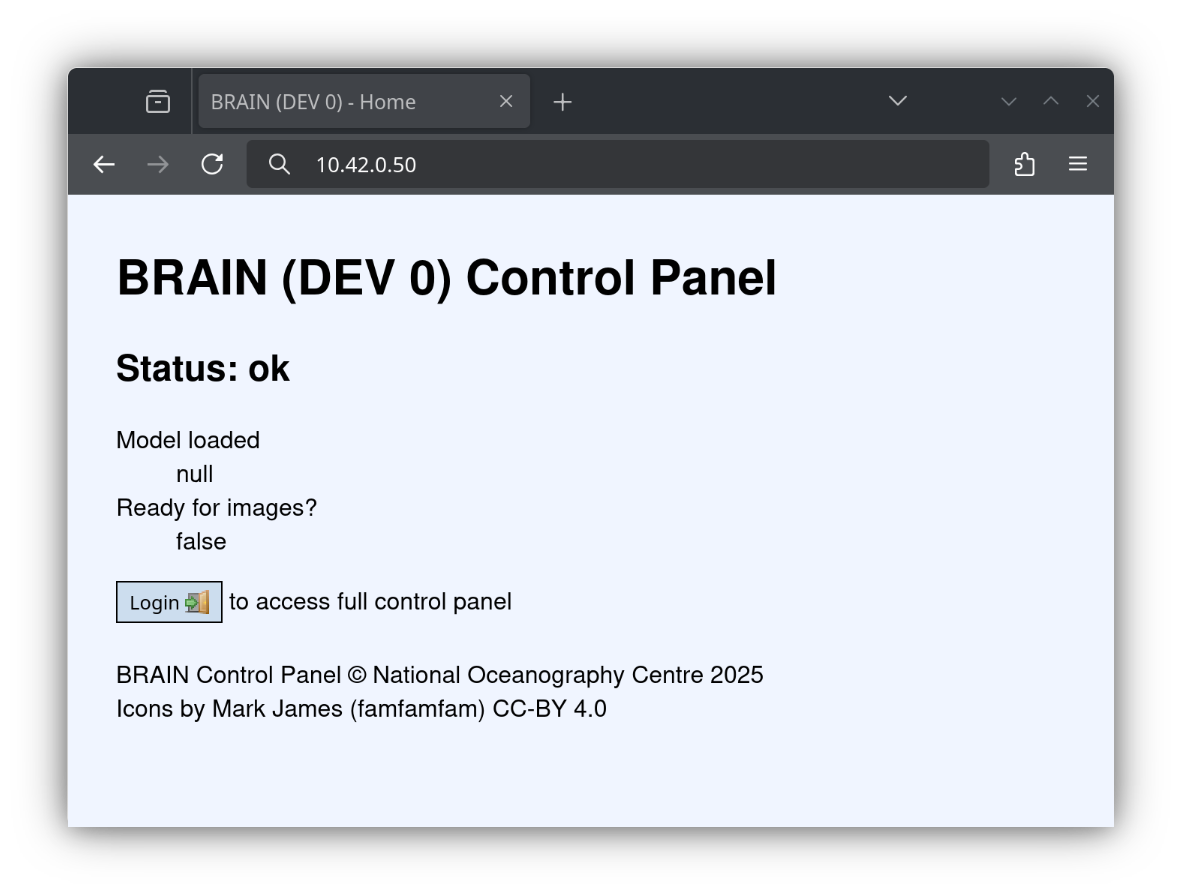
\includegraphics[width=0.75\textwidth]{brain-cpanel}
\caption{Initial screen of the BRAIN dashboard.}
\end{figure}

\newpage

\section{Configuring the BRAIN stack}

\newpage

\section{Debugging}

\subsection{Default network configuration}
\label{sec:debug-network_config}

The Ubuntu Server image ships with netplan by default, which will be configured by cloud-init to set the primary Ethernet port to be a DHCP client. By default \textbf{it locks this configuration to the MAC address seen on first boot}. This means that without removing the "match" line from /etc/netplan/50-cloud-init.yaml you will not be able to use the SD card interchangably on other Jetsons.

\subsection{Reflashing firmware}
\label{sec:debug-reflash_firmware}

With the software stack on the NVIDIA Jetsons being a little unstable, it's entirely possible to break the firmware from a simple software upgrade. There are a few different ways to reflash firmware on Jetson devices, but the  most reliable is to use the \texttt{flash.sh} tool supplied by Cannonical. NVIDIA's official instructions are to use the NVIDIA sdk-manager application, but I have found this to be extremely unreliable and time consuming.

Firmware for all Orin devices, including flash.sh can be found at \href{https://developer.nvidia.com/downloads/embedded/l4t/r36_release_v4.3/release/Jetson_Linux_r36.4.3_aarch64.tbz2}{https://developer.nvidia.com/downloads/embedded/l4t/r36\_release\_v4.3/release/Jetson\_Linux\_r36.4.3\_aarch64.tbz2}. The instructions below are derived from instructions found on \href{https://ubuntu.com/download/nvidia-jetson}{Ubuntu's NVIDIA Jetson download page}.

Run the following commands to set up your host machine for flashing.

\lstset{style=console}
\begin{lstlisting}
alewin@NOCS000000:~$ sudo apt install -y python3 mkbootimg bzip2 cpp device-tree-compiler
alewin@NOCS000000:~$ wget https://developer.nvidia.com/downloads/embedded/l4t/r36_release_v4.3/release/Jetson_Linux_r36.4.3_aarch64.tbz2
alewin@NOCS000000:~$ tar xf Jetson_Linux_R36.4.3_aarch64.tbz2 && cd Linux_for_Tegra/
alewin@NOCS000000:~$ sudo ./tools/l4t_flash_prerequisites.sh
\end{lstlisting}

You should now connect your computer to the USB C port next to the GPIO pins. You can only use this port for flashing firmware. The AGX has a dedicated "force recovery" button (this is the middle one of three). Hold this down while powering the device on. Once the light comes on, you may release the button. Now start to flash the firmware, for the AGX run:

\lstset{style=console}
\begin{lstlisting}
alewin@NOCS000000:~$ sudo ./flash.sh p3737-0000-p3701-0000-qspi internal
\end{lstlisting}

This command will take a long while (about 15 mins) and may appear to hang at times. Be patient, and it should eventually come back with success.

\subsection*{Side note specific to the Orin Nano}

One alternative method is to first boot the JetPack 5.1.3 SD card image (\href{https://developer.nvidia.com/downloads/embedded/l4t/r35_release_v5.0/jp513-orin-nano-sd-card-image.zip}{https://developer.nvidia.com/downloads/embedded/l4t/r35\_release\_v5.0/jp513-orin-nano-sd-card-image.zip}) and to use apt to update the firmware. This has had mixed results in the past and is not reccomended.

\subsection{Authenticating against the NVIDIA container repository}

For older versions of BRAIN, it was neccesary to set up API keys for NVIDIA's container repository. You can do this by signing up for an NVIDIA developer account, and proceeding to \href{https://org.ngc.nvidia.com/setup/api-keys}{https://org.ngc.nvidia.com/setup/api-keys}. Supply the bearer token as follows:

\lstset{style=console}
\begin{lstlisting}
deploy@brain:~$ docker login nvcr.io
Username: $oauthtoken
Password: <Your Key>
\end{lstlisting}

\printbibliography

\end{document}
